\DiaryEntry{The Pendulum, 1}{2019-01-15}{ODE}

We consider a friction-free pendulum of length $l$ with a point mass $m$ at the end. The ODE describing the displacement $\theta$ is given by

\bee
\frac{d^2\theta}{dt^2} + \frac{g}{l} \sin(\theta) = 0
\eee

For small displacement $\theta \ll 1$, we can approximate the sine function and obtain the linearized ODE

\bee
\frac{d^2\theta}{dt^2} + \frac{g}{l} \theta = 0
\eee

The Figure below shows traces ($\theta(t), \frac{d\theta}{dt}$) for a small displacement, $\theta_0 = 0.1, \frac{d\theta}{dt}(t=0) = 0$, with nonlinear and linearized ODE, respectively. No difference between the two ODEs can be seen.

\begin{figure}[H]
  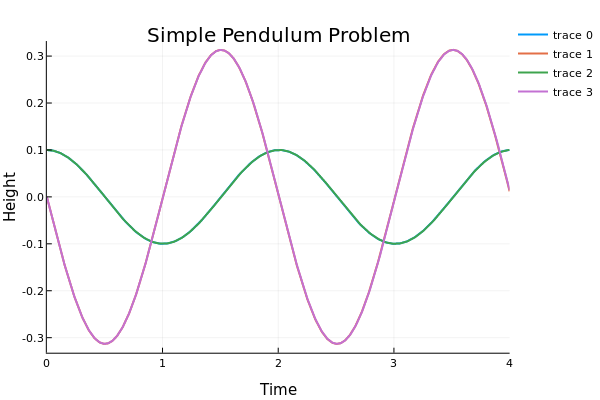
\includegraphics[scale=0.5]{images/pendulum_1_1.png}
\end{figure}

The following Figure shows the solution of the linearized ODEs for a small initial displacement $\theta_0 = 0.1, \frac{d\theta}{dt}(t=0) = 0$ and a large displacement $\theta_0 = 1.4, \frac{d\theta}{dt}(t=0) = 0$. Since the ODE is linear, the two solutions are different by a (time-constant) factor; the period of the two is the same, though.

\begin{figure}[H]
  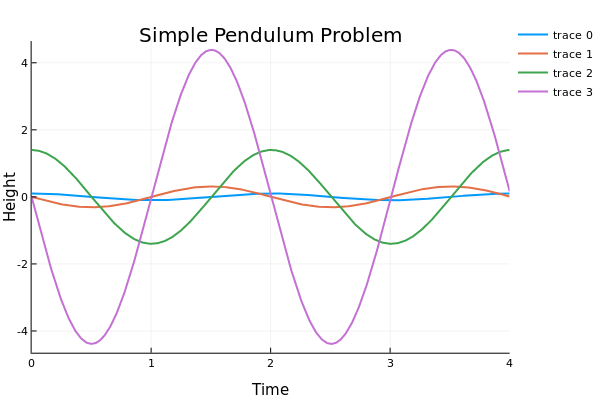
\includegraphics[scale=0.5]{images/pendulum_1_2.png}
\end{figure}


Finally, we compare the ODE solution and the linearized ODE soluton for a large initial displacement ($\theta_0=1.4$). The correct solution has a larger period than the solution of the linearized ODE.


\begin{figure}[H]
  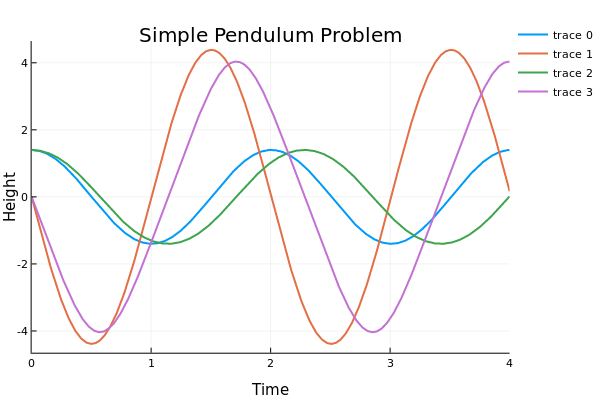
\includegraphics[scale=0.5]{images/pendulum_1_3.png}
\end{figure}



%%% Local Variables:
%%% mode: latex
%%% TeX-master: "journal"
%%% End:
